\section{Specification-Guided Input Abstraction}\label{sec:inpabs}

Systematic fuzzing of consensus protocols entails navigating an input space that is \textit{structurally vast yet semantically sparse}. A naive exploration of the raw byte space fails to generate valid state objects with high probability, while standard coverage-guided mutations struggle to penetrate the complex, inter-dependent validity checks that guard the core consensus logic. This challenge is exacerbated by the unforgiving nature of state serialization protocols (e.g., SSZ), where even semantically equivalent objects may diverge due to strict canonicalization rules.

To overcome this semantic gap, \tool decomposes the fuzzing process into two distinct phases: an offline \textit{abstraction phase} that constructs a high-fidelity semantic map of the input domain, and an online \textit{exploration phase} (detailed in \autoref{sec:fuzzing}) where a reinforcement learning agent navigates this map. In this section, we present the \textit{specification-guided input abstraction} (SGIA), the cornerstone of the offline phase. SGIA synthesizes a structured action space through the integration of static type analysis and dynamic constraint solving. This process constructs a finite set of abstract \emph{buckets} --- representing canonical forms, boundary conditions, and specific edge cases --- that serve as the fundamental primitives for the subsequent fuzzing loop.

\subsection{Type-Driven Input Partitioning}
\label{sec:type_partition}

The foundation of our abstraction is a partitioning derived from the intrinsic properties of the serialization schema's type system. This step establishes the structural substrate of the input domain.
Critically, the abstraction function $\varsigma(v)$ for a field $v$ does not return regions directly, but rather a set of \textit{partitioning thresholds}. These thresholds act as the skeletal framework of the domain, upon which finer semantic intervals are later constructed.

For each field $v$ of type $\tau$, $\varsigma(v)$ systematically maps the high-cardinality domain into a discrete set of pivot points, ensuring a baseline geometric coverage of the state space.

\begin{example}[Base Thresholds for Primitives]
Consider a field $v$ of type \icode{uint64}. Instead of arbitrary arithmetic sets, we select extrema and standard uniform pivots. Let $\icode{MAX} = 2^{64}-1$. The function $\varsigma(v)$ generates:
\[
\varsigma(v) = \{ 0, 1, {\sf MAX} \} \cup \left\{ \frac{k}{8} \cdot {\sf MAX} \;\middle|\; k \in \{1, \dots, 7\} \right\}.
\]
This creates 8 equidistant semantic regions alongside the critical boundary values. Similarly, for a sequence type \icode{List[T, N]}, the partition focuses on topological length boundaries:
\[ \varsigma(v) = \{ 0, 1, N-1, N \}. \]
These sets are later used to induce the concrete intervals (e.g., $[0, 0], (0, 1), [1, \frac{1}{8}{\sf MAX}), \dots$) for mutation.
\end{example}

By initializing the abstraction map $\Theta$ with these type-based thresholds (line 5 of \autoref{alg:abstraction}), \tool ensures that the exploration policy is cognizant of the fundamental structural limitations of the data format. A comprehensive catalog of supported types and their corresponding initial thresholds is provided in \autoref{apdx:typp}.

\begin{algorithm}[t]
    \caption{Specification-Guided Abstraction}
    \begin{algorithmic}[1]
    % \small
        \Procedure{\textsc{Partition}}{$\phi$; $k$, $n$}
            \State \textbf{input:} specification $\phi$
            \State \textbf{parameter:} subset size $k$, target threshold count $n$
            \State \textbf{output:} a set $\Theta$ of variable-thresholds pairs
            \State $\Theta \gets \{ v \mapsto \varsigma(v) \mid v \in {\sf vars}(\phi) \}$ \Comment{type-driven partitioning}
            \State $\Phi_0 \gets {\sf decompose}(\phi)$ \Comment{CNF decomposition into clauses}
            \State $\Phi \gets \bigcup_{\varphi \in \Phi_0} \beth(\varphi) $ \Comment{constraint tightening for clause}
            \While{$\sum_{v \in {\sf vars}(\Theta)} |\Theta[v]| < n$}
                \State $\Phi' \gets {\sf choose}(\Phi, k)$ \Comment{use a subset of $k$ clauses}
                \State $M \gets {\sf maximize}(\Phi', \Theta; \delta)$ \Comment{solving for best thresholds}
                \If {$\lnot {\sf UNSAT}(M)$} \Comment{found thresholds}
                    \State $\Theta \gets \{ v \mapsto \Theta[v] \cup \{ M[v] \} \mid v \in {\sf vars}(\Theta) \}$ \Comment{merge}
                \Else {\bf \ continue}
                \EndIf
            \EndWhile
            \State \Return $\Theta$
        \EndProcedure
    \end{algorithmic}
    \label{alg:abstraction}
\end{algorithm}

\subsection{Constraint-Guided Domain Refinement}
\label{sec:spec_derivation}

While type-driven partitioning provides a coarse structural map, it lacks insight into the semantic dependencies enforced by the consensus logic. To expose these hidden boundaries, \tool refines the domain using the formal specification. This refinement is achieved through an iterative algorithm, \textsc{Partition} (as shown in \autoref{alg:abstraction}), which systematically injects critical thresholds derived from protocol validity constraints.

The algorithm begins by initializing the abstraction map $\Theta$ with the base partitions (line 5). Building upon this substrate, the algorithm proceeds to refine the domain through three key stages: decomposition, constraint tightening, and iterative maximization.

\paragraph{Decomposition and tightening}
The refinement process first decomposes the monolithic specification $\phi$ into a set of atomic constraint clauses $\Phi_0$ (line 6). Typically, $\phi$ is converted into conjunctive normal form (CNF), where each clause represents a distinct validation rule.
To probe the exact edges of these feasible regions, we apply a \textit{constraint tightening operator}, denoted as $\beth$ (line 7). Formally, let an atomic constraint be $f(\mathbf{x}) \bowtie c$, where $\bowtie \in \{ \le, <, \ge, >, =, \neq \}$. The tightening operator is defined as:
\[
\beth(f(\mathbf{x}) \bowtie c) = 
\begin{cases} 
\{ f(\mathbf{x}) = c, \quad f(\mathbf{x}) = c + 1 \} & \text{if } \bowtie \in \{ \le, > \} \\
\{ f(\mathbf{x}) = c - 1, \quad f(\mathbf{x}) = c \} & \text{if } \bowtie \in \{ <, \ge \} \\
\{ f(\mathbf{x}) = c, \quad f(\mathbf{x}) = c \pm 1 \} & \text{if } \bowtie \in \{ =, \neq \}
\end{cases}.
\]
This operator explicitly distinguishes between the \textit{satisfying boundary} (the limit of validity) and the \textit{violating boundary} (the onset of invalidity).

\begin{example}[Constraint Tightening]
We illustrate the operator with both single-variable ($\varphi_0$) and multi-variable ($\varphi_1$) constraints:
\[
\begin{aligned}
\varphi_0 &: z < L  & \Rightarrow \quad & \beth(\varphi_0) = \{ z = L - 1, \quad z = L \}, \\
\varphi_1 &: x + y < M & \Rightarrow \quad & \beth(\varphi_1) = \{ x + y = M - 1, \quad x + y = M \}.
\end{aligned}
\]
These equations force the solver to locate values exactly on the geometric surfaces that separate valid and invalid states.
\end{example}

\paragraph{Geometric intuition of subset solving}
Ideally, we would solve the conjunction of all tightened constraints to find the exact vertices of the valid polytope. However, the complexity of the combined constraints often makes this computationally intractable. A key insight, illustrated in \autoref{fig:boundaries}, is that the critical boundary points (vertices) of a high-dimensional polytope are locally defined by the intersection of a small subset of hyperplanes.

\begin{figure}[t]
    \centering
    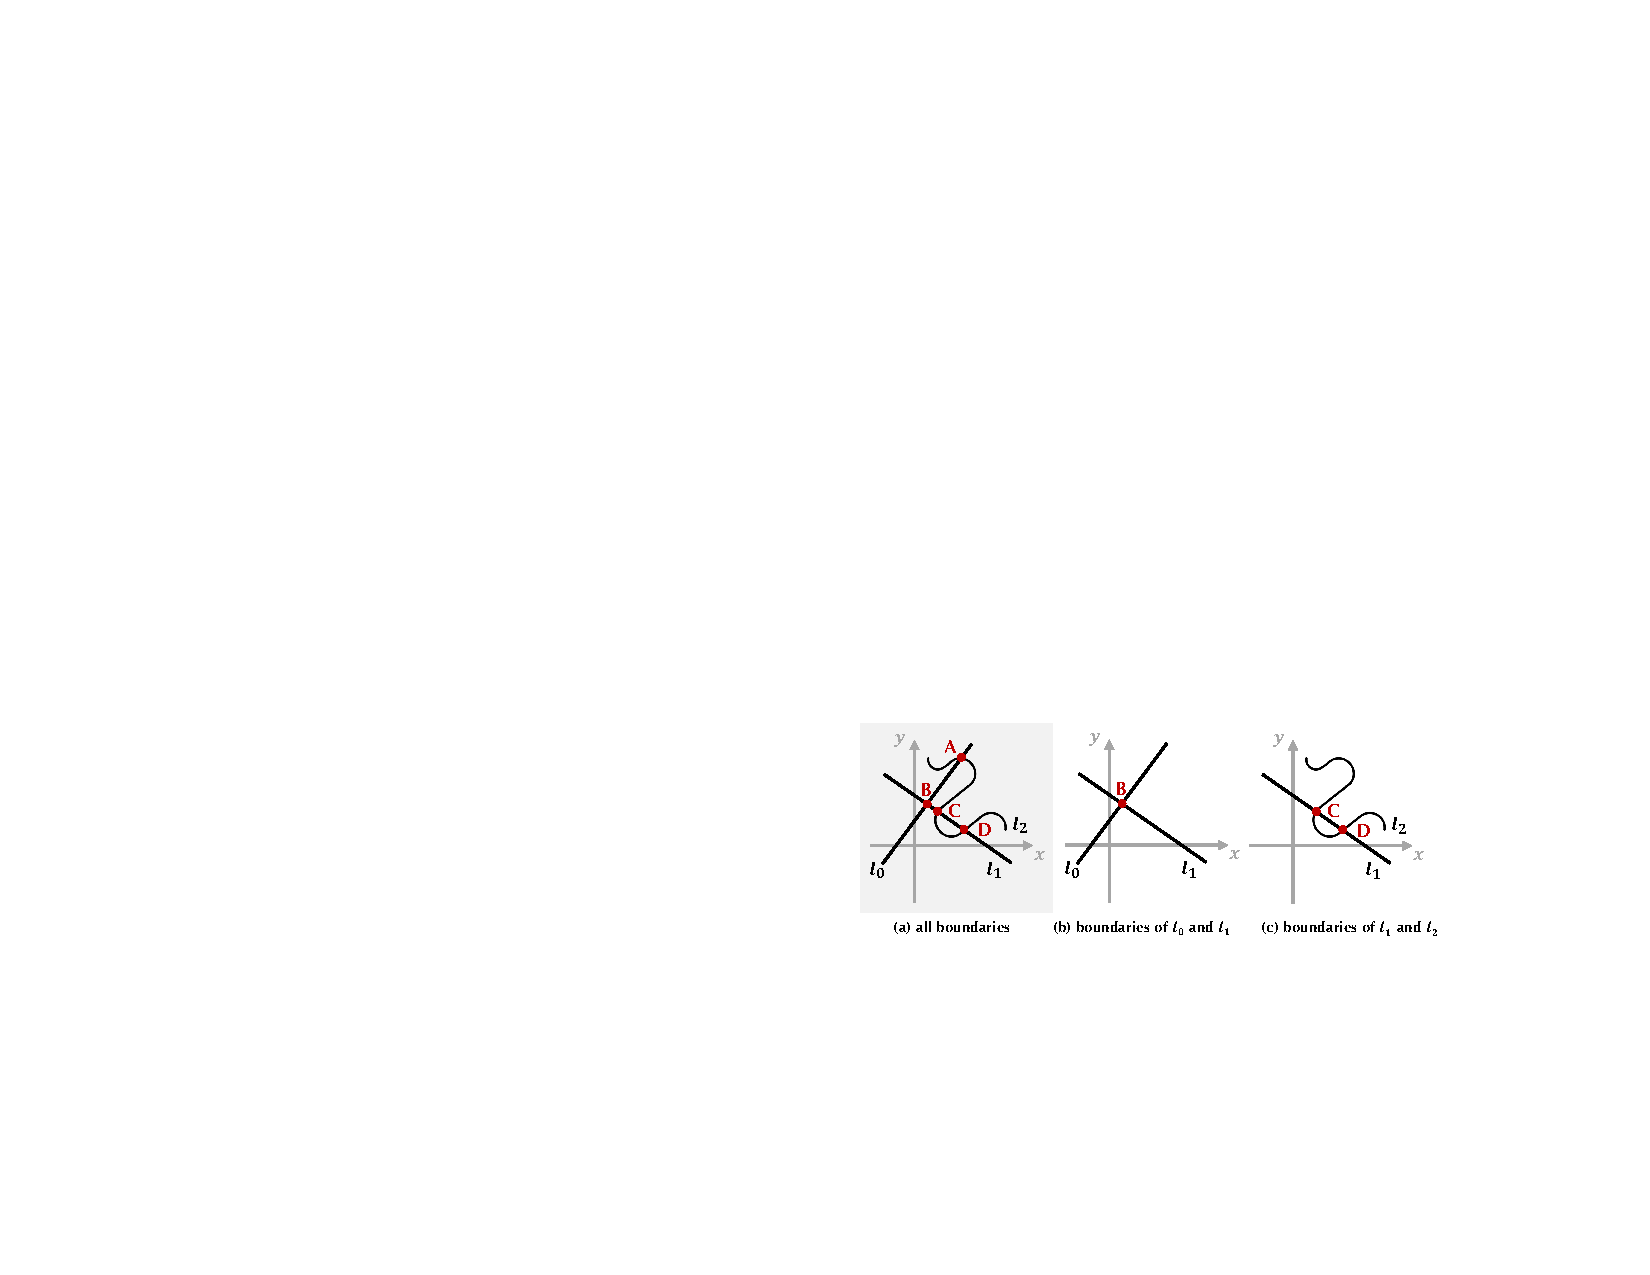
\includegraphics[width=\linewidth]{figs/boundaries.pdf}
    \caption{Geometric interpretation of subset constraint solving. The critical points $(A, B, C, D)$ are intersections of constraints $l_0, l_1, l_2$. Solving a subset of constraints, e.g., $\{l_0, l_1\}$ in (b), precisely recovers the associated vertex (B) without requiring the global complexity of the full system.}
    \label{fig:boundaries}
\end{figure}

As shown in \autoref{fig:boundaries} (b), solving a subset of constraints (i.e., $\{l_0, l_1\}$) is sufficient to pinpoint the specific vertex B, identical to its position in the full system in \autoref{fig:boundaries} (a). Even though the global constraint $l_2$ is ignored in this local view, the derived solution remains a valid geometric anchor of the state space.
Leveraging this property, \tool employs a \emph{randomized} constraint subsetting strategy. In each iteration, we select a random subset of $k$ clauses (line 9). Any solution to this subset guarantees a valid coordinate on some hyperplane of the input domain, significantly reducing solver overhead while preserving geometric fidelity.

\paragraph{Dispersion-based maximization}
While subset solving identifies candidate boundaries, multi-variable constraints often possess infinite solutions along a hyperplane. A naive solver might repeatedly return clustered or trivial values. To enforce solution diversity and maximize domain coverage, we augment the solver query with a \textit{dispersion metric} $\delta$ (line 10):
\[
    \delta(M, \Theta) = \min_{v \in {\sf vars}(M), u \in \Theta[v]} | M[v] - u |.
\]
Geometrically, this metric represents the \textit{minimum clearance} between the candidate solution and the existing abstraction grid. By maximizing $\delta$, the solver is forced to locate the centroid of the largest unexplored region on the selected hyperplane. This maximin strategy ensures that new thresholds are topologically distinct from existing ones, effectively scattering the partition points to cover the geometry of the feasible region uniformly.

\paragraph{Threshold merging}
Valid solutions found by the solver are treated as critical \textit{partitioning thresholds} and merged into the abstraction map $\Theta$ (line 12). This effectively slices the coarse type-based buckets into finer, semantically significant intervals.

\begin{example}[Refined Interval Partitioning]
Suppose the type-based abstraction for a variable $x$ is initially $[0, {\sf MAX}]$. If the iterative refinement discovers two critical thresholds $t_1=10$ and $t_2=20$, the abstraction map $\Theta[x]$ is updated to partition the domain into five semantic buckets:
\begin{itemize}
    \item Thresholds: $\{10, 20\}$
    \item Intervals: $[0, 10], [10, 20], [20, {\sf MAX}]$
\end{itemize}
This allows the fuzzer to explicitly target the boundary values or sample from the specific regions between them.
\end{example}

This process repeats until the abstraction reaches the target granularity $n$, yielding a structured, spec-derived action space for the fuzzing agent.

By converting raw specifications into a structured set of semantic buckets, SGIA effectively constructs a high-fidelity map of the protocol's state space. This static abstraction serves as the foundation for our dynamic analysis. In the following section, we describe how \tool's exploration phase utilizes this map, employing reinforcement learning to identify the most promising boundaries for exposing consensus discrepancies.
